\documentclass[conference]{IEEEtran}
\IEEEoverridecommandlockouts
\usepackage{cite}
\usepackage{amsmath,amssymb,amsfonts}
\usepackage{algorithmic}
\usepackage{graphicx}
\usepackage{textcomp}
\usepackage{xcolor}
\usepackage{hyperref}
\setlength{\parskip}{0pt}
\setlength{\abovecaptionskip}{2pt}
\setlength{\belowcaptionskip}{2pt}
% tighten space around floats to keep the paper within the 6-page limit
\setlength{\textfloatsep}{1.15\baselineskip plus 0.2\baselineskip minus 0.4\baselineskip}
\setlength{\floatsep}{0.7\baselineskip plus 0.2\baselineskip minus 0.2\baselineskip}
\setlength{\intextsep}{0.7\baselineskip plus 0.2\baselineskip minus 0.2\baselineskip}
\setlength{\dbltextfloatsep}{1.15\baselineskip plus 0.2\baselineskip minus 0.4\baselineskip}
\setlength{\dblfloatsep}{0.7\baselineskip plus 0.2\baselineskip minus 0.2\baselineskip}
\def\BibTeX{{\rm B\kern-.05em{\sc i\kern-.025em b}\kern-.08em
    T\kern-.1667em\lower.7ex\hbox{E}\kern-.125emX}}

\begin{document}

\title{Safety Violation Detection in Educational Institutions: A Systematic Bibliometric Review of Deep Learning and Computer Vision Approaches}

\author{
\IEEEauthorblockN{Zhuldyz Basheyeva}
\IEEEauthorblockA{\textit{School of Software Engineering}\\
\textit{Astana IT University}\\
Astana, Kazakhstan\\
zhuldyz.basheyeva@astanait.edu.kz}
\and
\IEEEauthorblockN{Medet Akhmetov}
\IEEEauthorblockA{\textit{School of Software Engineering}\\
\textit{Astana IT University}\\
Astana, Kazakhstan\\
255388@astanait.edu.kz\\
\textit{(Corresponding author)}}
\and
\IEEEauthorblockN{Symbat Nurgaliyeva}
\IEEEauthorblockA{\textit{Department of Computer Engineering}\\
\textit{Astana IT University}\\
Astana, Kazakhstan\\
symbat.nurgaliyeva@astanait.edu.kz}
}

\maketitle

\begin{abstract}
Deep learning and computer vision techniques are increasingly proposed for automated detection of safety violations---violence, anomalous behavior, and weapons---in educational surveillance footage. This review synthesizes 50 peer-reviewed publications (2022--2026) through a hybrid systematic-bibliometric methodology following PRISMA 2020, combining keyword co-occurrence network analysis with CiteSpace burst detection. Four thematic clusters were identified: (C1) deep learning architectures for spatiotemporal feature extraction, (C2) temporal and motion analysis, (C3) application and deployment, and (C4) cross-cutting methods. ``Deep learning'' (23 occurrences) forms the central network hub, with ``violence detection'' (19) and ``anomaly detection'' (16) as primary application nodes. A shift toward lightweight, edge-deployable architectures---YOLO-family detectors and MobileNet-based extractors---characterizes 2025--2026. The central finding is a critical shortage of child-specific annotated datasets, limited geographic diversity, and a near-total absence of privacy-aware design. Six research directions are proposed: child-specific benchmarks, privacy-preserving architectures, multimodal fusion, lightweight edge optimization, cross-domain robustness evaluation, and human-in-the-loop alert integration.
\end{abstract}

\begin{IEEEkeywords}
deep learning, violence detection, anomaly detection, computer vision, video surveillance, educational safety, bibliometric analysis, systematic review
\end{IEEEkeywords}

\section{Introduction}

\subsection{Relevance of the Topic}

School violence, physical bullying, and concealed weapon possession continue to be reported globally, underscoring the limitations of traditional manual surveillance~\cite{b1,b2}. CCTV systems are now ubiquitous in schools, yet most rely on passive recording or human operators monitoring dozens of screens---a task for which humans are ill-suited due to fatigue and limited attention~\cite{b3,b4,b26}. In parallel, deep learning architectures have demonstrated remarkable capabilities in extracting patterns from video data~\cite{b5,b6,b7}, catalyzing research at the intersection of automated video analysis and public safety~\cite{b8,b9,b10}.

\subsection{Literature Gap}

Despite this progress, several critical gaps persist. First, the majority of existing studies focus on general-purpose public surveillance---streets, transit hubs, and stadiums---with comparatively limited attention devoted to the unique constraints of educational environments~\cite{b11,b12}. Second, many state-of-the-art models rely on computationally expensive architectures that are impractical for deployment in schools with limited hardware budgets~\cite{b13,b14}. Third, there is a notable scarcity of child-specific annotated datasets for training and evaluating detection models, as most benchmark corpora feature adult subjects in generic settings~\cite{b15,b16}. Fourth, the ethical and privacy implications of deploying AI-based surveillance on minors remain underexplored in the technical literature. This review makes three distinctive contributions: (1) the first systematic-bibliometric synthesis of deep-learning-based safety violation detection focused on educational institutions; (2) a data-driven research landscape mapping via keyword co-occurrence networks, thematic clustering, and citation burst analysis; and (3) foregrounding of child-specific concerns---privacy, dataset bias, and age-appropriate modeling---absent from existing surveys.

\subsection{Research Goal and Questions}

This review provides a structured synthesis of deep learning and computer vision research for safety violation detection in educational settings, guided by four research questions:

\begin{enumerate}
\item \textbf{RQ1}: What deep learning architectures and computer vision techniques are most commonly applied to detect safety violations in educational settings?
\item \textbf{RQ2}: What datasets and evaluation protocols dominate the current literature, and what are their limitations for child-focused applications?
\item \textbf{RQ3}: What thematic clusters and temporal trends characterize this emerging research domain?
\item \textbf{RQ4}: What are the principal challenges and future directions for deploying these systems in real-world educational environments?
\end{enumerate}

\section{Methodology}

\subsection{Review Design}

This study employs a hybrid systematic-bibliometric design. The systematic component follows PRISMA 2020 for literature identification, screening, and eligibility; the bibliometric component uses keyword co-occurrence network analysis and CiteSpace burst detection to map the research domain's intellectual structure.

\subsection{Search Strategy}

Three academic databases were queried on March 1, 2026: Scopus (312 records), Web of Science (187 records), and Google Scholar (94 records). The query combined three Boolean blocks: \textit{("violence detection" OR "anomaly detection" OR "weapon detection" OR "firearm detection") AND ("deep learning" OR "machine learning" OR "computer vision" OR "CNN" OR "YOLO") AND ("school" OR "educational" OR "campus" OR "surveillance" OR "CCTV")}. The temporal scope encompassed 2022--2026, capturing the period following widespread adoption of YOLOv5 and transformer-based architectures.

\subsection{Inclusion and Exclusion Criteria}

Studies were included if they: (a) applied ML/CV methods to violence, anomaly, or weapon detection in surveillance contexts; (b) were peer-reviewed with full methodological exposition; (c) were published in English between 2022--2026; and (d) had accessible full text. Studies using non-ML/CV methods, addressing unrelated domains, published before 2022, lacking full text, or limited to abstracts were excluded.

\subsection{Study Selection Process}

The initial search across three databases returned 593 records. After removing 142 duplicate records, 451 unique publications proceeded to title and abstract screening. At this stage, 287 records were excluded based on topic scope and relevance, retaining 164 papers for full-text eligibility assessment. Full-text eligibility assessment excluded 114 papers: 38 used non-ML/CV methods, 31 addressed unrelated domains, 22 predated 2022, 15 lacked accessible full text, and 8 were abstracts only. The final corpus comprised 50 studies included in both the qualitative synthesis and bibliometric analysis (Fig.~\ref{fig:prisma}).

\begin{figure}[t]
\centerline{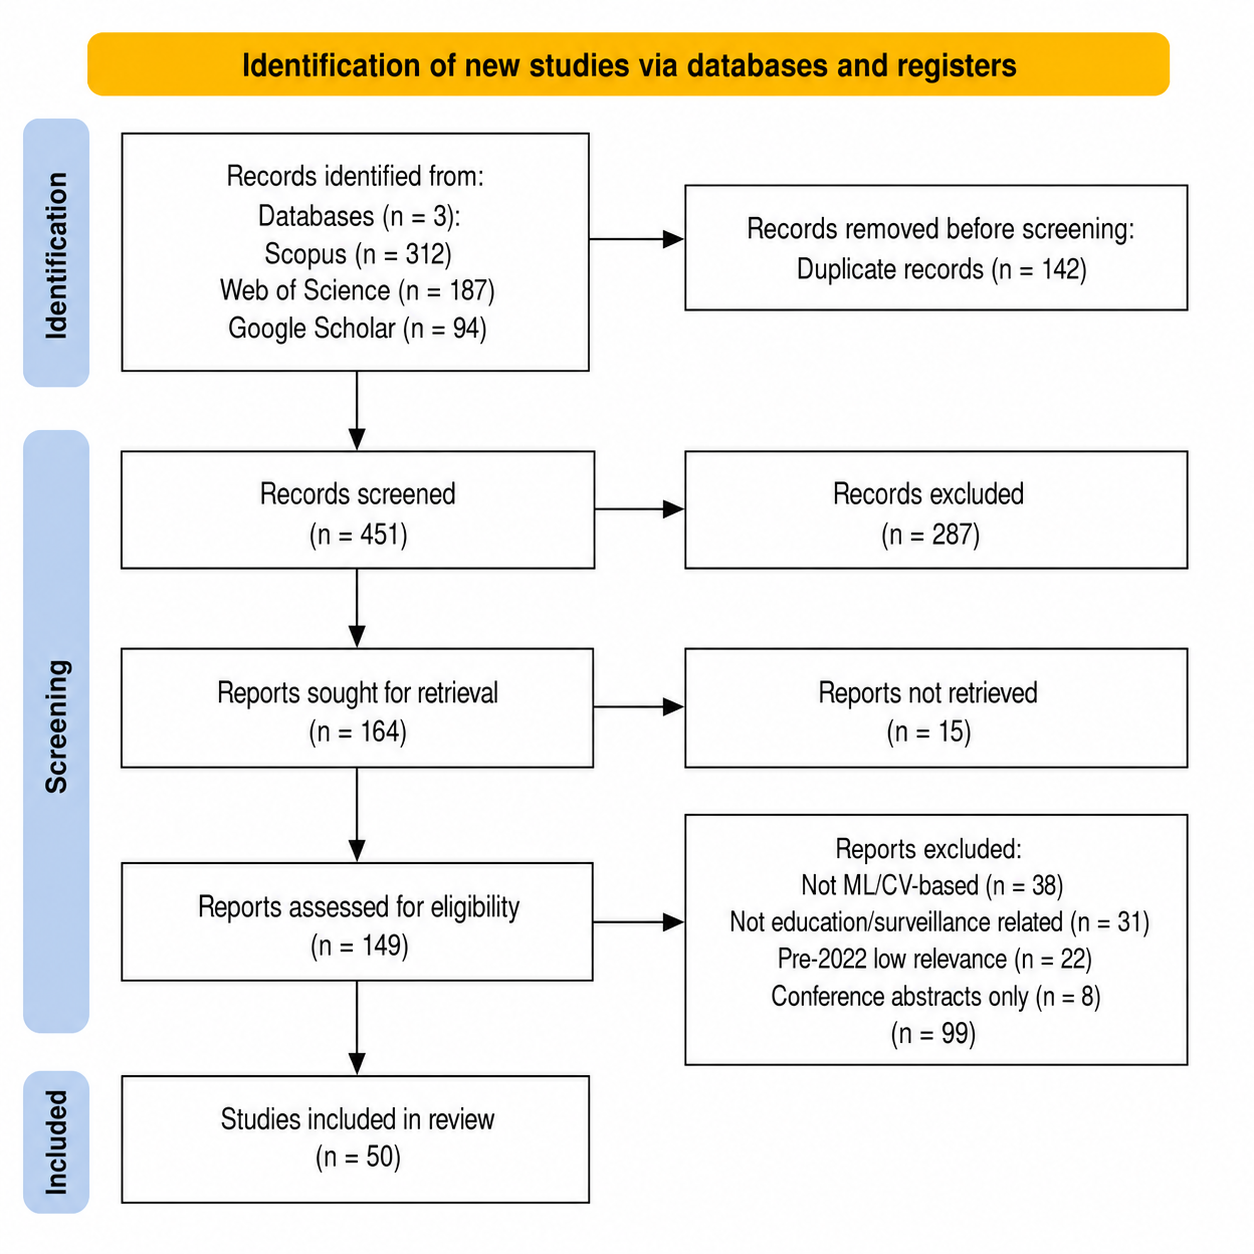
\includegraphics[width=0.55\columnwidth]{Prisma/prisma_diagram.png}}
\caption{PRISMA 2020 flow diagram of the study selection process.}
\label{fig:prisma}
\end{figure}

\subsection{Data Extraction and Analysis}

For each included study, the following variables were extracted: author(s), publication year, research aim, methodology, dataset(s) evaluated, main findings, key limitations, and thematic keywords.

Keywords were extracted from titles and abstracts using a curated vocabulary of 30 terms across four categories: Architecture, Temporal/Motion, Application/Deployment, and Methods/Cross-cutting. Co-occurrence matrices were constructed to model the frequency with which keyword pairs appeared within the same paper. ``Convolutional neural network'' and ``CNN'' were treated as separate entries to capture papers using the abbreviated versus full form, but were conceptually grouped for cluster interpretation; similarly, ``video surveillance'' and ``CCTV'' were retained as distinct terms with different connotations.

Thematic clusters were identified through a two-stage process: (1) the keyword co-occurrence network was partitioned using community detection (modularity maximization) to identify natural groupings; (2) content analysis of full-text methodology sections validated and refined the computationally derived groupings. Studies were assigned to clusters based on primary methodological contribution: novel architecture design (C1), motion and temporal modeling (C2), deployment-oriented systems (C3), or cross-cutting method improvement (C4). Research trends were identified through three complementary analyses: temporal overlay visualization colored by average publication year, CiteSpace burst detection, and manual longitudinal reading of the 50 full texts to corroborate computationally detected trends.

\subsection{Tools}

Bibliometric visualizations were generated using Python-based implementations of network analysis (NetworkX) and kernel density estimation (SciPy), producing outputs analogous to VOSviewer and CiteSpace. The PRISMA flowchart was rendered using Matplotlib. All analytical scripts, the literature analysis matrix, and output files are publicly available at: \url{https://github.com/marioscordia/disser}.

\subsection{Quality Assurance and Limitations}

The review process followed PRISMA 2020 standards. Methodological limitations include: (a) restriction to Scopus, Web of Science, and Google Scholar---IEEE Xplore and ACM Digital Library were excluded because Scopus indexes a substantial portion of their proceedings, providing partial coverage overlap, though niche workshops indexed exclusively in those databases may have been missed; (b) exclusion of non-English publications; (c) single-reviewer screening without inter-rater reliability assessment and reliance on a curated keyword vocabulary.

\section{Results}

\subsection{Corpus Overview}

The systematic search and PRISMA-guided screening process identified 50 studies for both qualitative synthesis and bibliometric analysis. Table~\ref{tab:years} presents the distribution by publication year.

\begin{table}[t]
\caption{Distribution of Included Studies by Year}
\begin{center}
\renewcommand{\arraystretch}{1.0}
\begin{tabular}{|c|c|c|}
\hline
\textbf{Year} & \textbf{Pub.} & \textbf{Share} \\
\hline
2022 & 10 & 20\% \\
2023 & 14 & 28\% \\
2024 & 11 & 22\% \\
2025 & 12 & 24\% \\
2026 & 3 & 6\% \\
\hline
\textbf{Total} & \textbf{50} & \textbf{100\%} \\
\hline
\end{tabular}
\label{tab:years}
\end{center}
\end{table}

The included studies span a range of publication venues, with MDPI journals accounting for the largest share, followed by IEEE Access, Elsevier, and Springer venues. Of the 50 studies, 10 (20\%) directly address safety violation detection in educational institutions or involve child-specific analysis; the remaining 40 (80\%) focus on general public-space surveillance but were retained for methodological transferability.

\subsection{Publication Trends}

Scopus contributed 44 studies (88\%) and Web of Science 6 (12\%), peaking in 2023 (14 publications) with sustained output through 2024--2025 (Fig.~\ref{fig:trend}). Google Scholar contributed 94 records but none survived after deduplication and screening; its role was limited to broadening the initial search net.

\subsection{Keyword Co-occurrence Analysis}

Fig.~\ref{fig:keyword-network} illustrates the keyword co-occurrence network. ``Deep learning'' (23 occurrences) is the central hub, with ``violence detection'' (19) and ``anomaly detection'' (16) as primary application nodes, and ``convolutional neural network'' (15), ``CNN'' (15), and ``LSTM'' (10) as the dominant architectural terms.

\begin{figure}[t]
\centerline{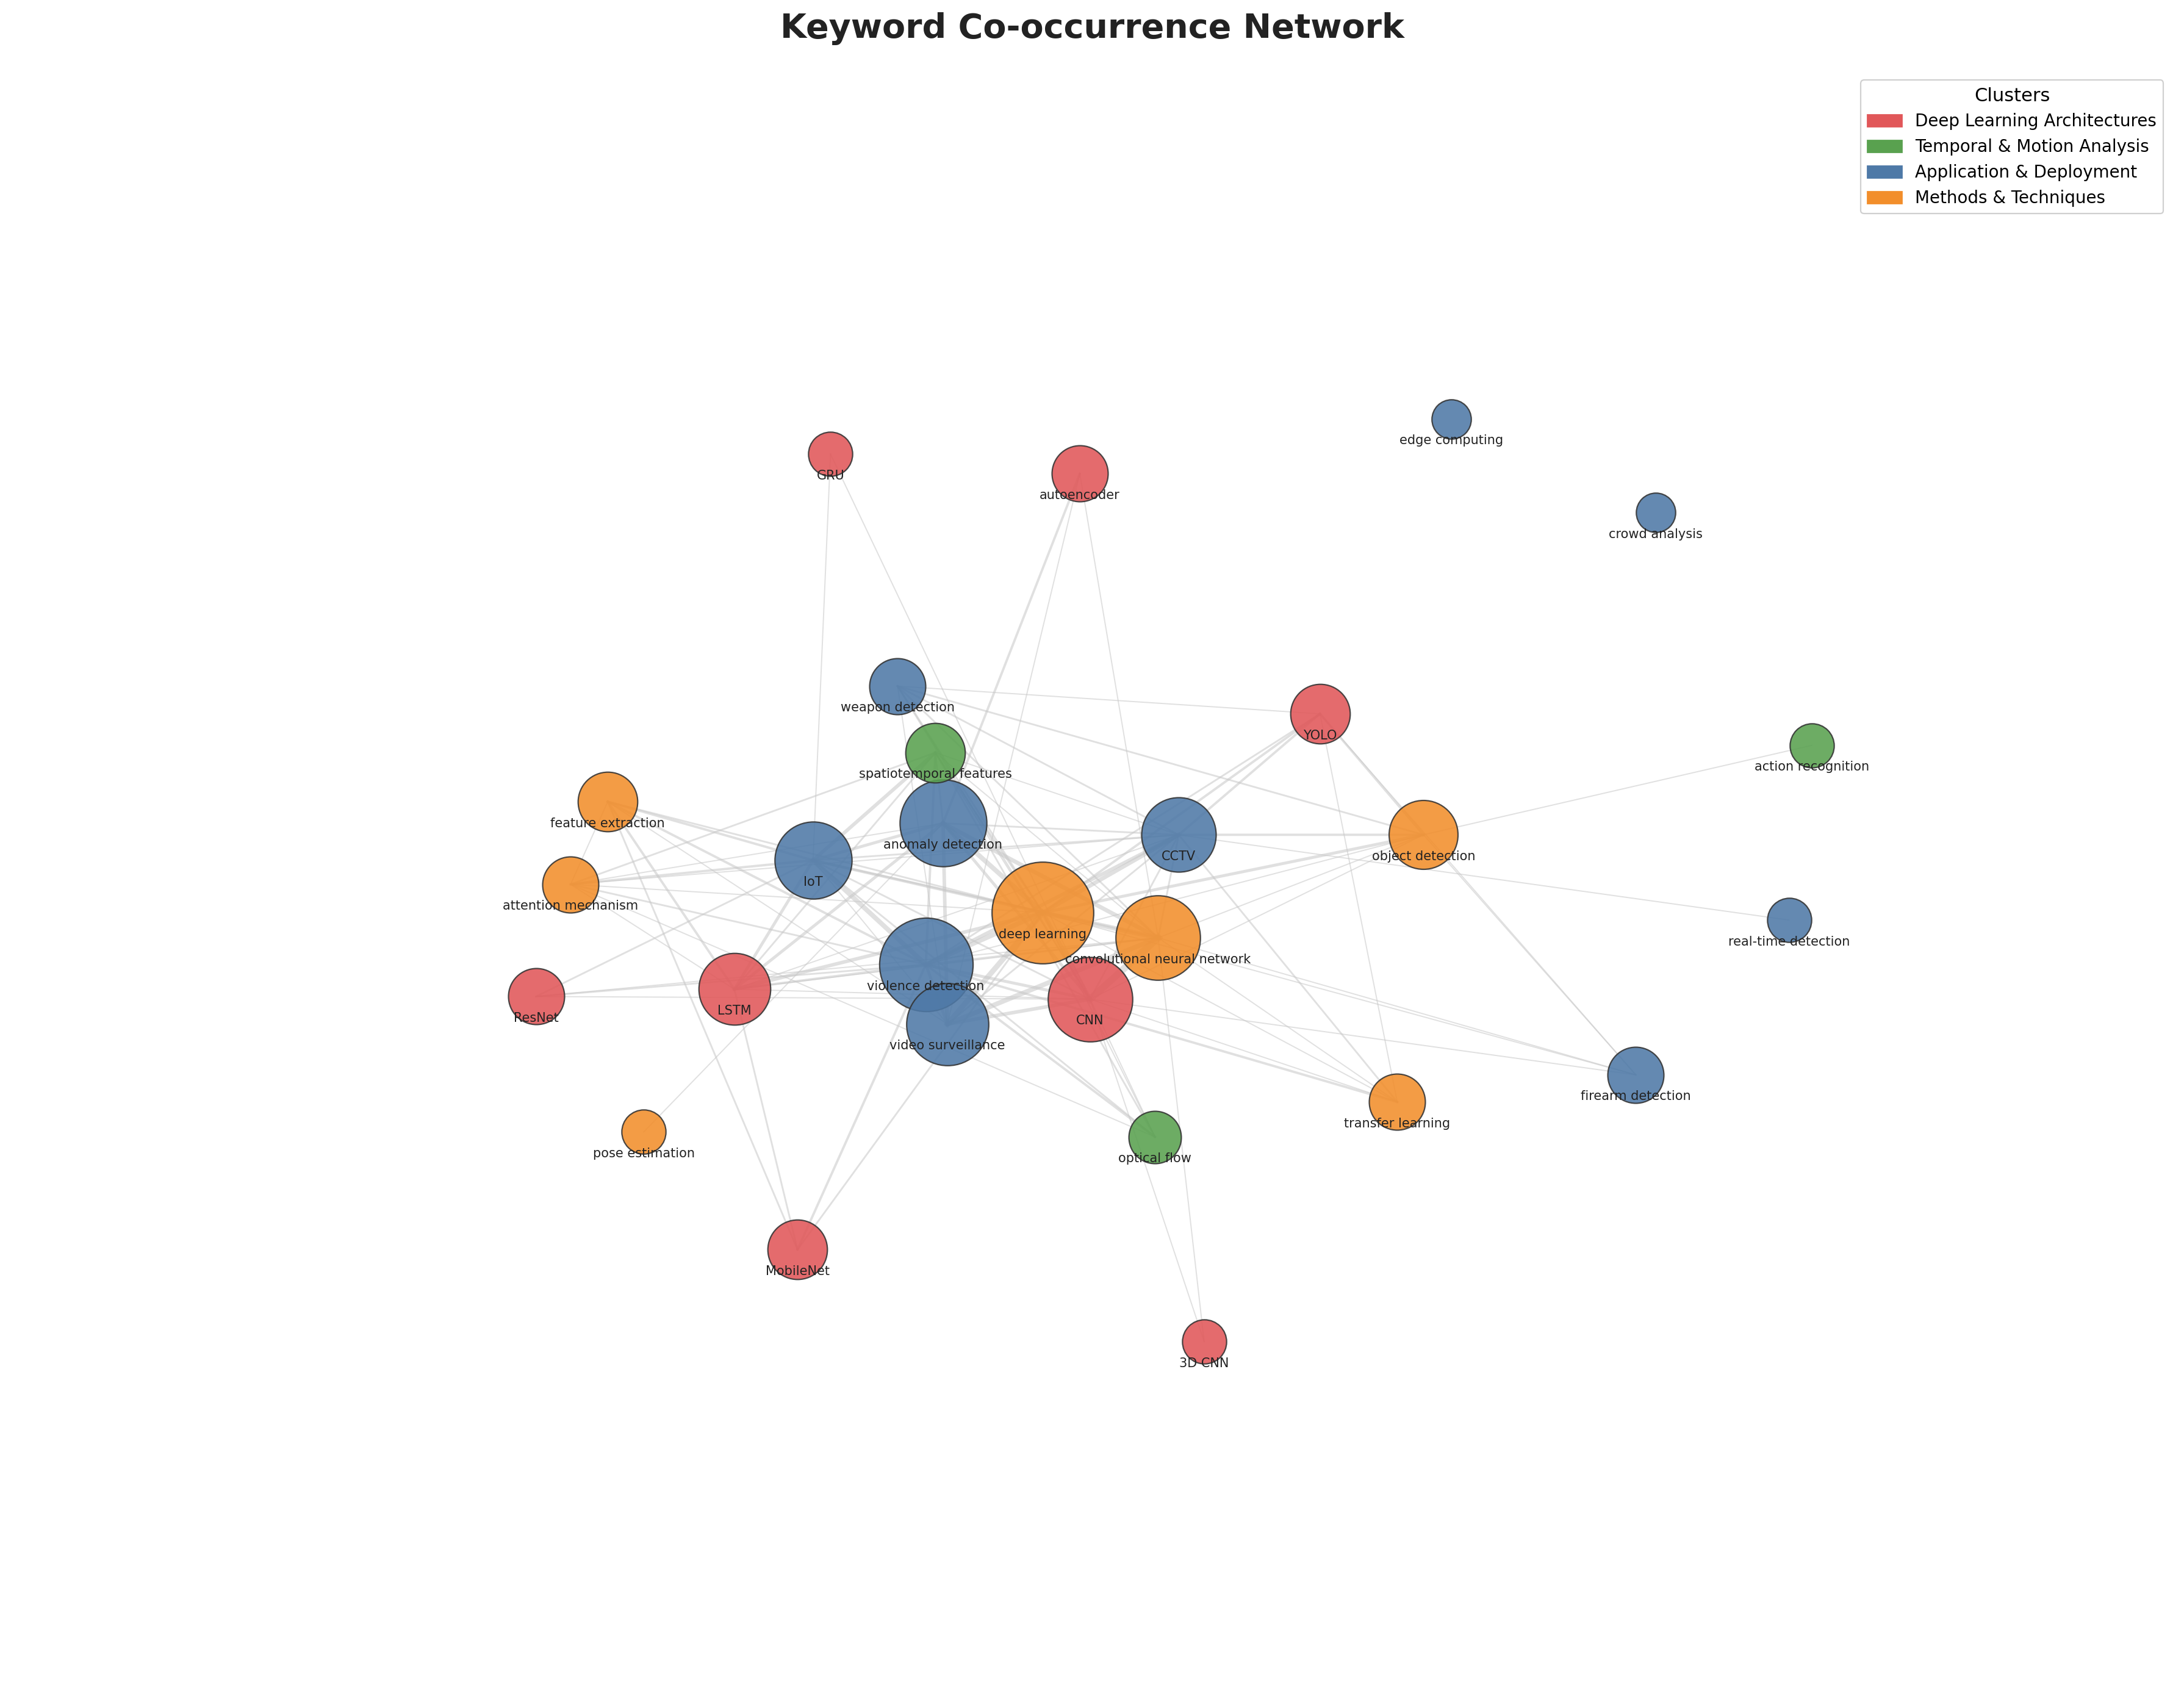
\includegraphics[width=\columnwidth]{VOSViewer/vosviewer_keyword_network.png}}
\caption{Keyword co-occurrence network (node size = frequency).}
\label{fig:keyword-network}
\end{figure}

The temporal overlay (Fig.~\ref{fig:overlay}) shows the most recent keyword activity concentrated in 2025--2026 around pose estimation, optical flow, firearm detection, and MobileNet, whereas the earliest activity---edge computing, ResNet, and weapon detection---dates to 2022--2023.

\begin{figure}[t]
\centerline{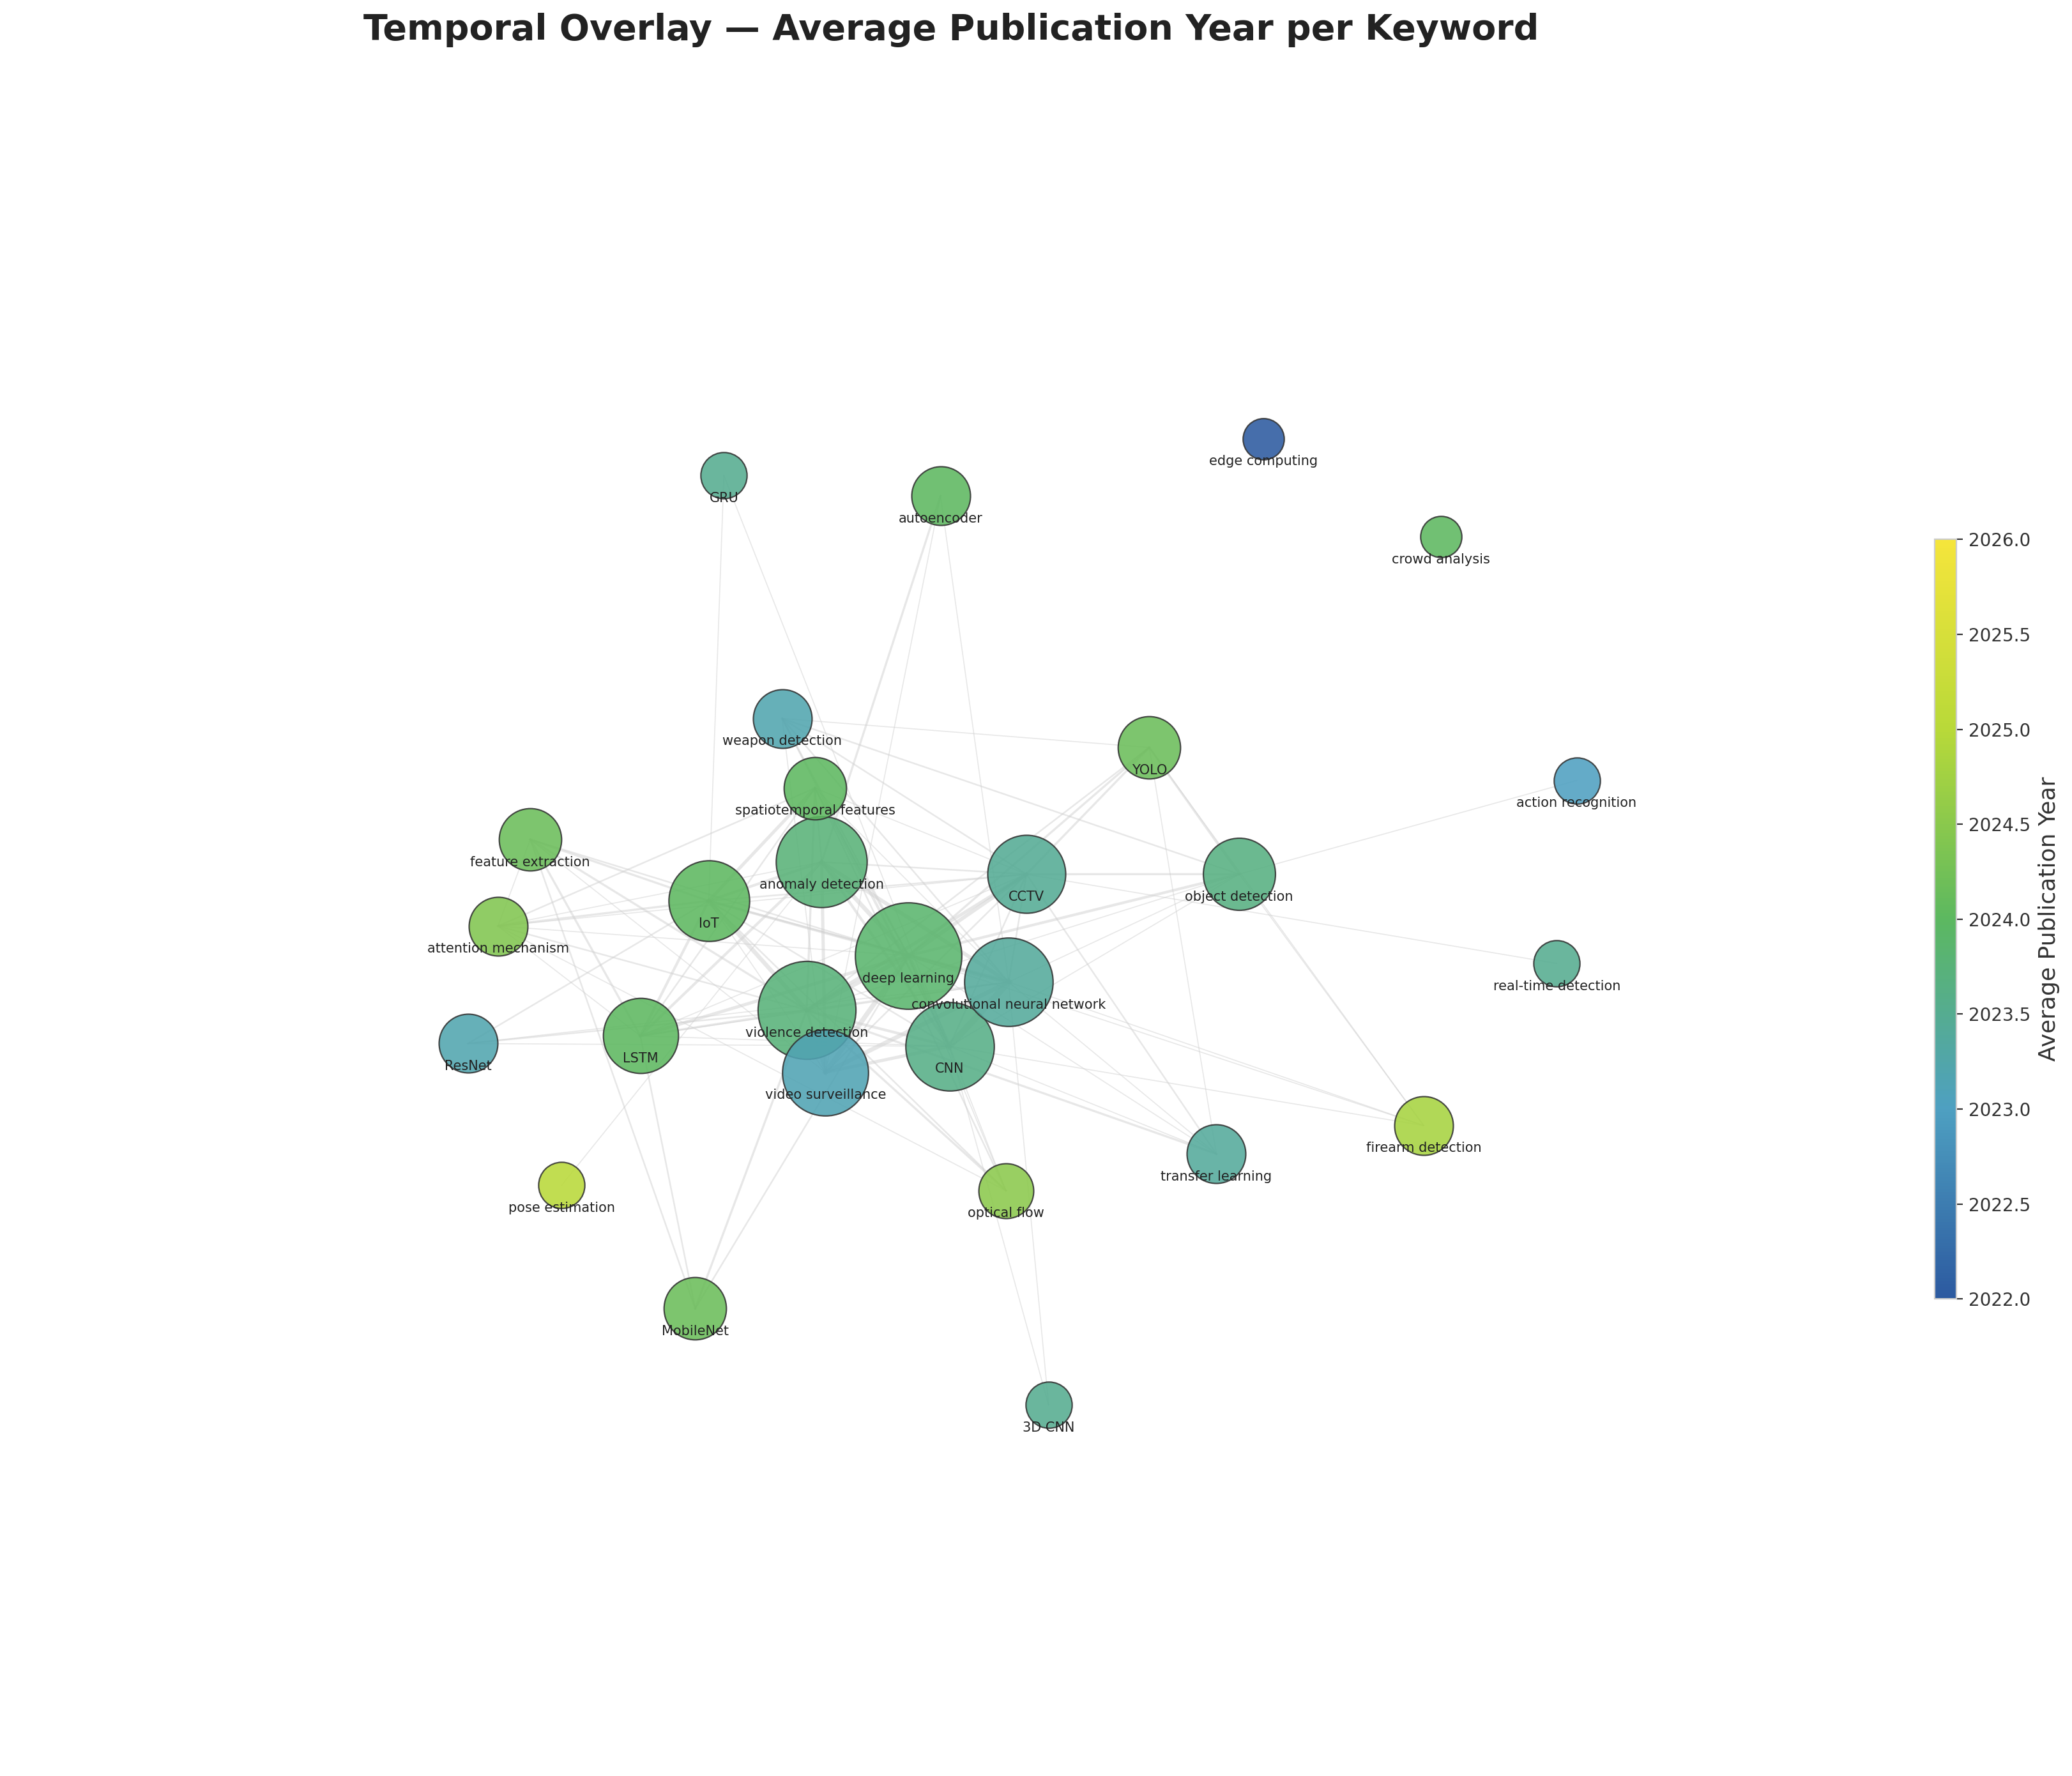
\includegraphics[width=\columnwidth]{VOSViewer/vosviewer_overlay.png}}
\caption{Temporal overlay (blue = 2022--2023, yellow = 2025--2026).}
\label{fig:overlay}
\end{figure}

Top keywords by frequency: \textit{deep learning} (23), \textit{violence detection} (19), \textit{anomaly detection} (16), \textit{convolutional neural network} and \textit{CNN} (15 each), \textit{video surveillance} (14), \textit{IoT} (12), \textit{CCTV} (11), \textit{LSTM} (10), \textit{object detection} (9).

\subsection{Thematic Clusters}

Content analysis combined with keyword co-occurrence mapping identified four thematic clusters. Table~\ref{tab:clusters} presents the cluster structure.

\begin{table*}[t]
\caption{Thematic Clusters in Safety Violation Detection Research}
\begin{center}
\scriptsize
\setlength{\tabcolsep}{3pt}
\renewcommand{\arraystretch}{1.15}
\begin{tabular}{|c|p{2.2cm}|p{5.0cm}|p{5.0cm}|}
\hline
\textbf{C} & \textbf{Title} & \textbf{Common Characteristics} & \textbf{Summary of Key Findings} \\
\hline
C1 & Deep Learning Architectures & Studies designing, comparing, or optimizing neural network topologies (CNN, LSTM, GRU, ResNet, MobileNet, YOLO, 3D CNN, autoencoder) for spatiotemporal feature extraction & Hybrid architectures integrating 3D convolutions or pre-trained 2D CNNs with recurrent units and attention mechanisms consistently exceed 90\%, with the strongest hybrid architectures surpassing 95\%, on controlled benchmarks; lightweight variants maintain competitive performance with reduced computational requirements \\
\hline
C2 & Temporal and Motion Analysis & Studies emphasizing motion representation---optical flow, spatiotemporal feature engineering, action/behavior recognition, skeleton-based pose estimation & Optical flow-based statistical features enable 2D CNNs to achieve performance comparable to 3D CNNs; skeleton-based approaches using pose estimation abstract away from appearance-based biases, relevant for child-specific applications \\
\hline
C3 & Application and Deployment & Studies focused on real-world deployment in surveillance contexts (CCTV, IoT, edge computing, crowd analysis) with emphasis on real-time performance & YOLO-family architectures (v5--v8) achieve real-time throughput on commodity and edge hardware (NVIDIA Jetson Nano) with weapon detection mAP exceeding 90\%; IoT-integrated systems report end-to-end pipelines from detection to automated alerting \\
\hline
C4 & Methods and Techniques & Studies bridging architecture and application through transfer learning, attention mechanisms, feature extraction, pose estimation, and object detection & Attention mechanisms deliver improvements of 2--4\% over non-attention baselines; transfer learning from ImageNet pre-trained models reduces data requirements; multimodal fusion (RGB + optical flow + audio) outperforms unimodal approaches by approximately 2\% average precision \\
\hline
\end{tabular}
\label{tab:clusters}
\end{center}
\end{table*}

The four clusters map to the research questions. C1 addresses RQ1 by cataloging neural network topologies for safety violation detection; C2 isolates temporal modeling as a distinct sub-problem where motion-centric approaches achieve competitive results with lighter backbones; C3 speaks to RQ4 by grouping deployment-oriented studies around YOLO detectors, IoT pipelines, and edge hardware; C4 functions as a cross-cutting toolkit---transfer learning, attention, and feature extraction improve performance irrespective of architecture, explaining C4's high between-cluster connectivity.

\subsection{Citation Burst Analysis}

The burst analysis (Fig.~\ref{fig:citespace-burst}) shows ``LSTM'' with sustained burst activity across 2022--2026 as a foundational technique; ``deep learning,'' ``feature extraction,'' and ``MobileNet'' exhibit bursts concentrated in 2025, while ``violence detection,'' ``IoT,'' ``YOLO,'' ``spatiotemporal features,'' and ``attention mechanism'' burst in 2024. The earliest bursts---``CCTV'' and ``object detection''---appear in 2022, with ``anomaly detection,'' ``CNN,'' and ``video surveillance'' following in 2023.

\begin{figure}[t]
\centerline{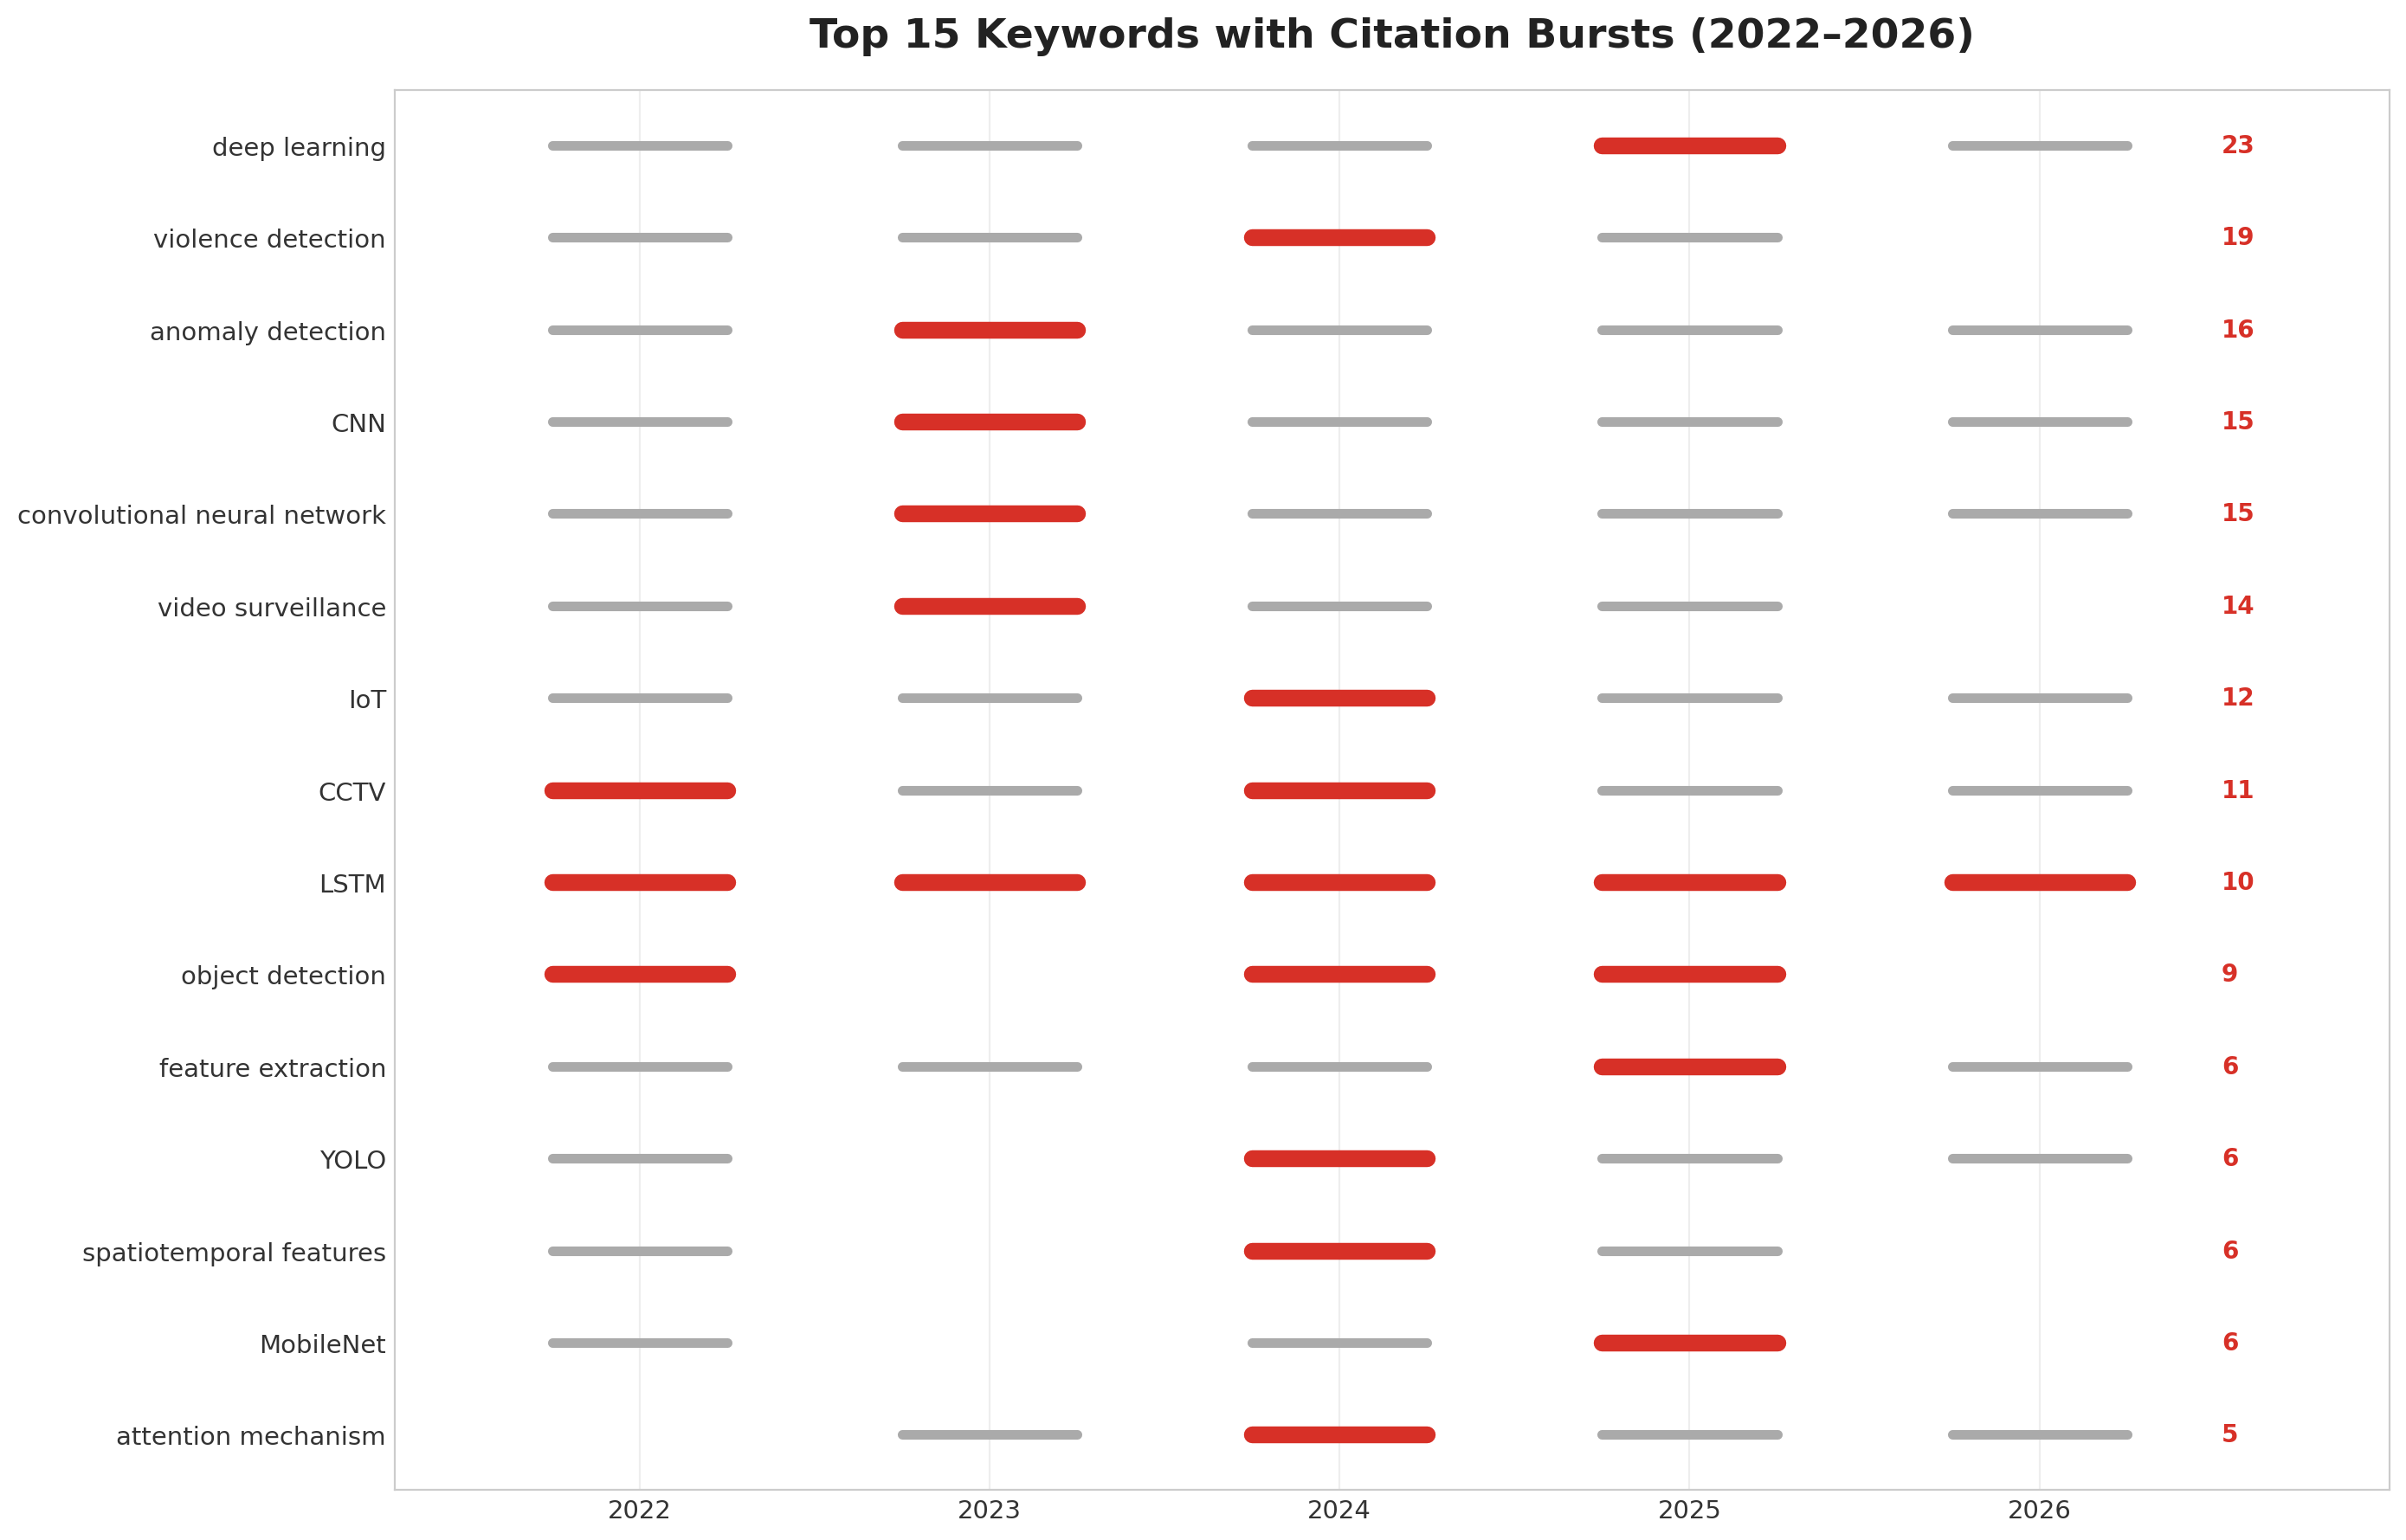
\includegraphics[width=\columnwidth]{Citespace/citespace_burst_timeline.png}}
\caption{Top 15 keywords with the strongest citation bursts --- red segments indicate heightened activity.}
\label{fig:citespace-burst}
\end{figure}

\begin{figure}[t]
\centerline{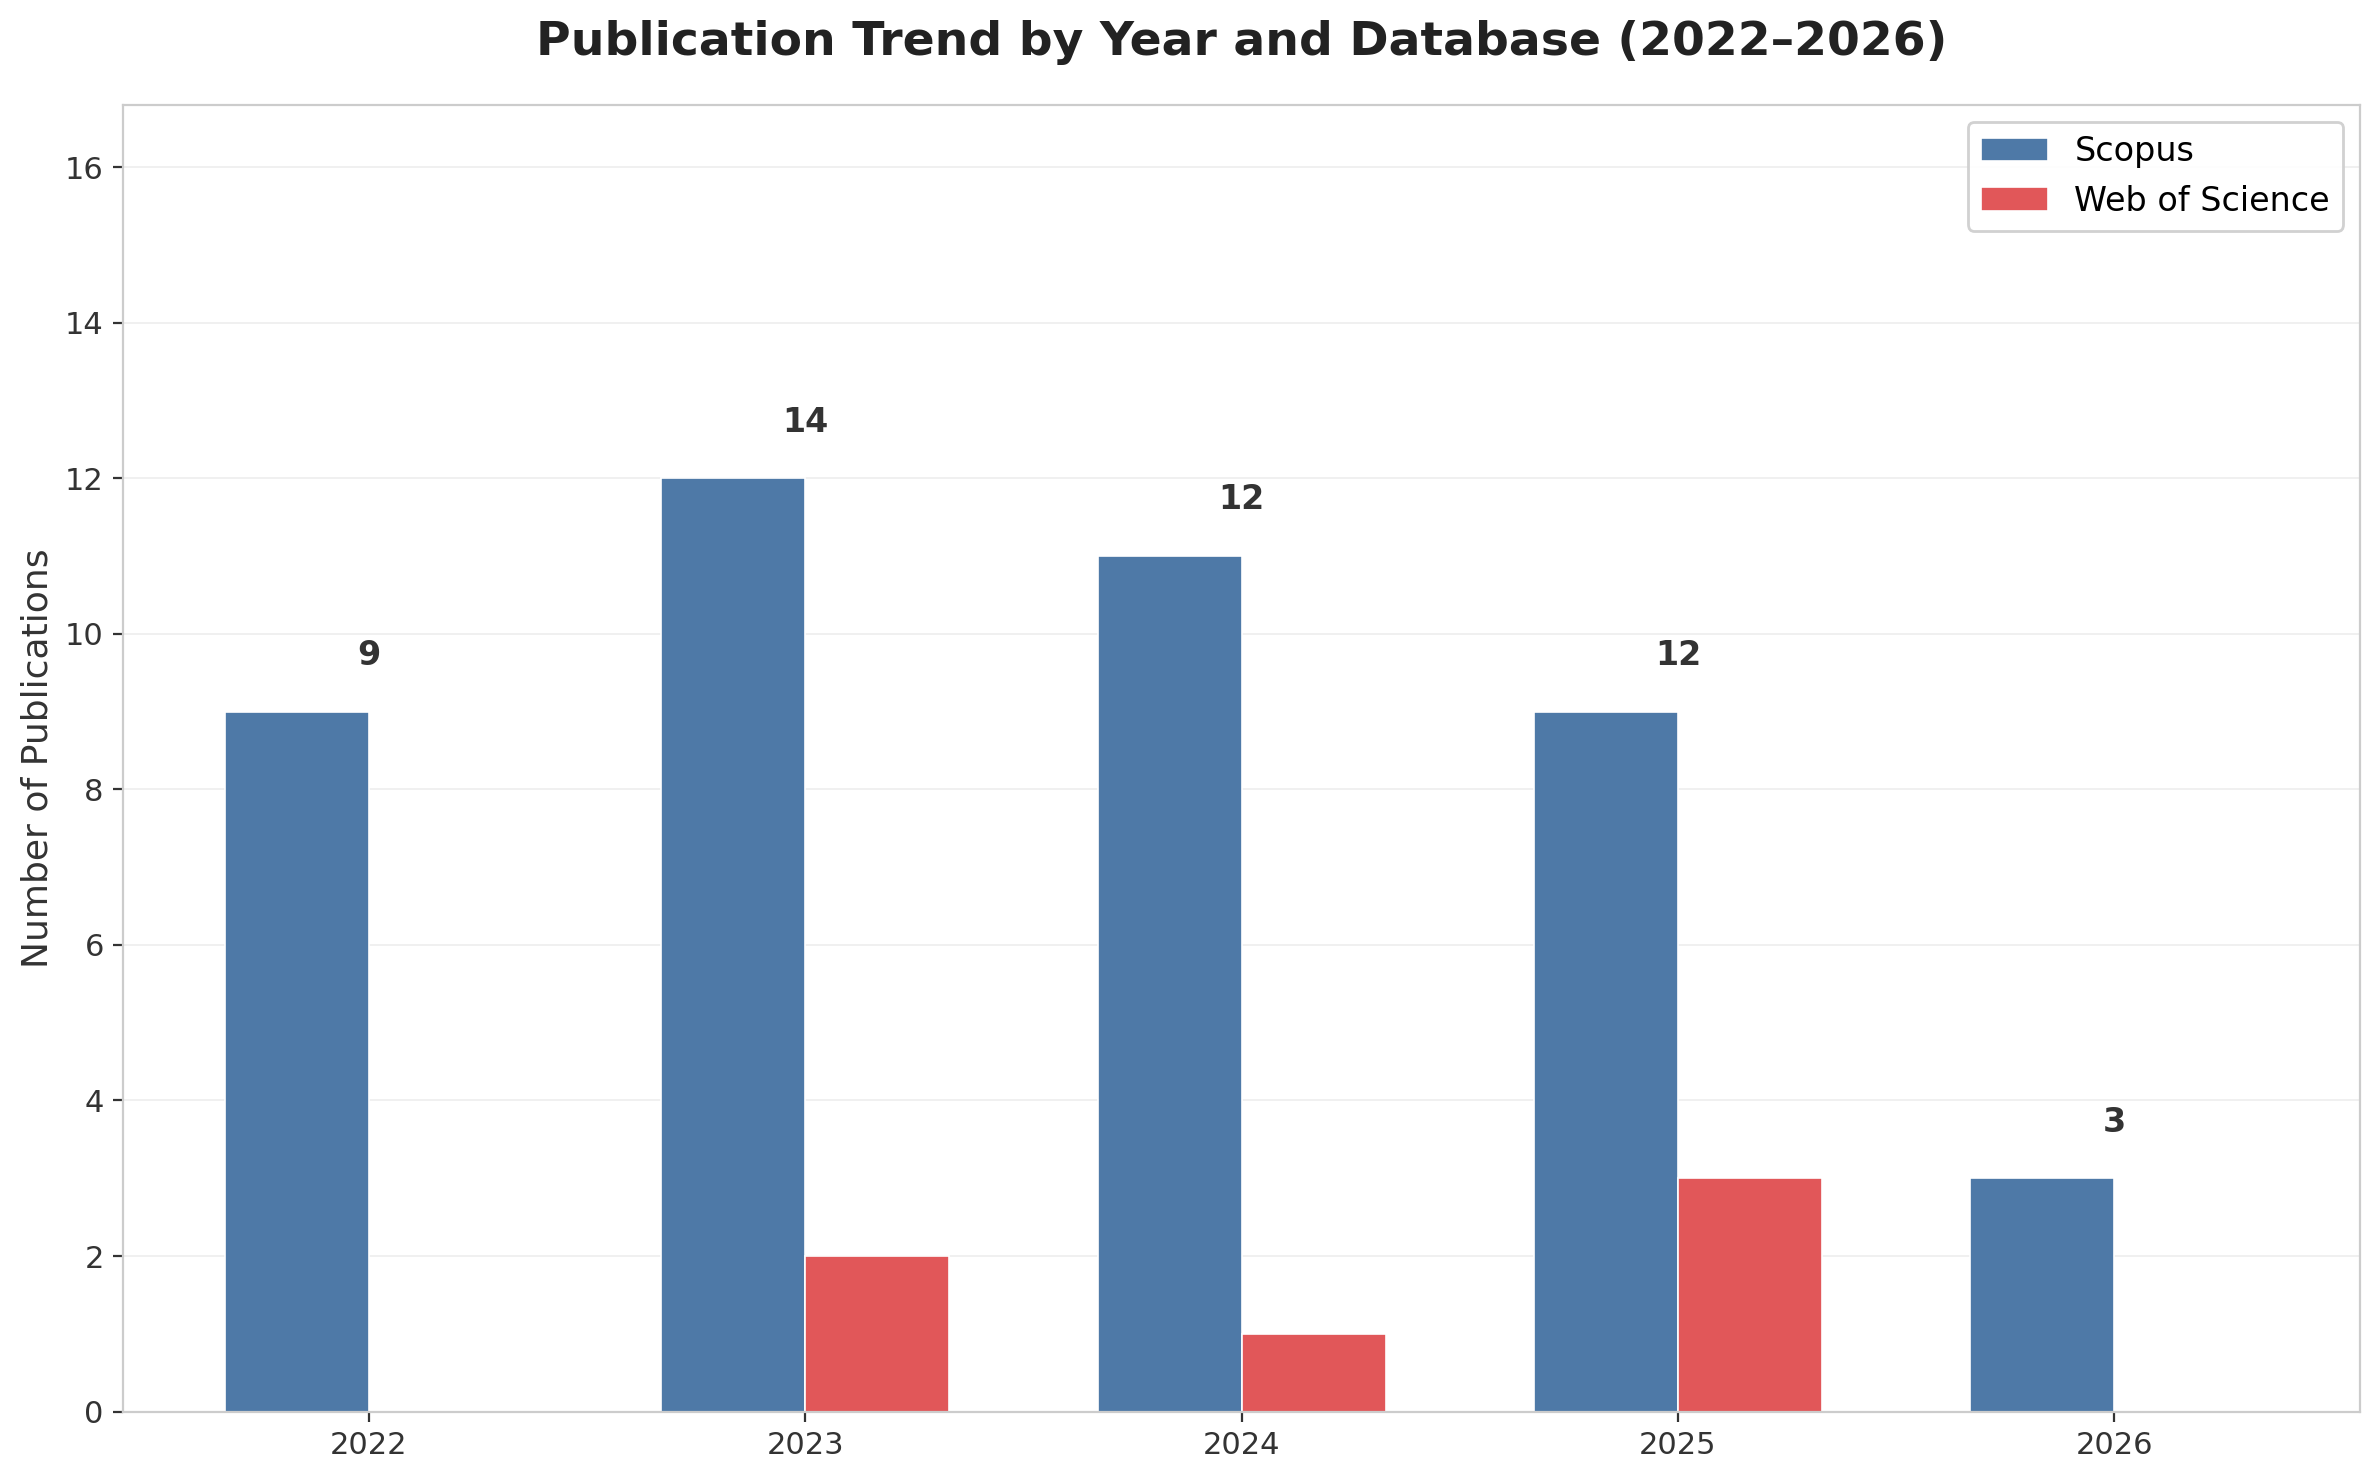
\includegraphics[width=0.92\columnwidth]{Citespace/citespace_trend.png}}
\caption{Annual publication trend by database (2022--2026).}
\label{fig:trend}
\end{figure}

\subsection{Literature Matrix Summary}

The literature analysis matrix provides a structured overview of all 50 studies. Accuracy and AUC dominate evaluation metrics (44 of 50 studies); UCF-Crime, ShanghaiTech Campus, and Hockey Fights are the most frequent benchmarks, all featuring adult subjects in public-space settings---only two studies provide child-specific data (CABAD~\cite{b15} and Daily School Break~\cite{b11}), confirming the gap under RQ2. The limitation profile varies by cluster: C1 studies cite computational complexity, C3 note environmental robustness, and C4 identify dataset generalizability, reflecting each cluster's distinct research focus.

\begin{table}[t]
\caption{Representative Model Performance. \textsuperscript{\textbf{†}}Studies addressing educational or child-specific settings.}
\begin{center}
\scriptsize
\setlength{\tabcolsep}{2pt}
\renewcommand{\arraystretch}{1.1}
\begin{tabular}{|p{2.1cm}|p{2.0cm}|p{1.0cm}|p{1.8cm}|c|c|}
\hline
\textbf{Study} & \textbf{Architecture} & \textbf{Task} & \textbf{Dataset} & \textbf{Metric} & \textbf{Score} \\
\hline
Le\'{o}n et al. (2026)~\cite{b1} & CNN + YOLO & Weapon & — & Acc. & 99\% \textbf{†} \\
\hline
Singh et al. (2025)~\cite{b6} & AE + Pose & Weapon & — & F1 & 86\% \\
\hline
Mukto et al. (2024)~\cite{b3} & YOLO + MobileNet & Violence & — & Acc. & 97\% \\
\hline
Perseghin \& Foresti (2023)~\cite{b11} & CNN & Violence & Daily School Break & Acc. & 95\% \textbf{†} \\
\hline
Kozhamkulova et al. (2023)~\cite{b2} & MoveNET & Violence & — & Acc. & 98\% \textbf{†} \\
\hline
Jebur et al. (2023)~\cite{b18} & ResNet & Violence & RLVS & Acc. & 41\% \\
\hline
\end{tabular}
\label{tab:model-performance}
\end{center}
\end{table}

\section{Discussion}

\subsection{Interpretation of Key Findings}

The four thematic clusters reveal a field organized around a central tension: architectural sophistication versus deployability. C1 (Architectures) emphasizes accuracy maximization through increasingly complex networks; C3 (Application and Deployment) privileges real-time throughput and hardware efficiency via lightweight YOLO and MobileNet variants. This tension is visible in the temporal evolution: the overlay visualization places the earliest activity in deployment-oriented and architectural terms---edge computing and ResNet (2022--2023)---and the most recent in lightweight and pose-based approaches such as MobileNet and pose estimation (2025--2026). The CNN--LSTM paradigm, observed in 26 of 50 studies, indicates consensus that effective video anomaly detection requires integrating spatial feature extraction with temporal sequence modeling; the recent growth in attention mechanisms suggests movement beyond naive concatenation toward more sophisticated feature weighting~\cite{b5,b17}.

\subsection{Cross-Cluster Comparative Analysis}

Deep learning underpins all four clusters. C2 and C4 function as methodological bridges: C2's motion strategies provide the temporal understanding that C1 and C3 depend upon, while C4's transfer learning and attention mechanisms enhance performance across all clusters. Few studies address the intersection of lightweight architectures (C1/C3) with skeleton-based child-specific modeling (C2).

First, the accuracy--efficiency trade-off: C1's deep CNN-LSTM ensembles exceed 90\% accuracy (best surpassing 95\%) yet require GPU-class hardware; C3 achieves real-time edge inference at marginally lower accuracy. Second, the role of appearance: C2's motion-centric approaches suppress appearance to avoid bias, while C4's techniques are appearance-driven. Reconciling these through dynamic multimodal fusion remains open.

\subsection{Most Effective Methods}

Hybrid architectures combining 3D or pre-trained 2D CNNs with recurrent units (LSTM, BiLSTM, GRU) and attention mechanisms achieve the strongest performance, with accuracies exceeding 90\% (strongest surpassing 95\%) on controlled benchmarks~\cite{b17,b18,b2}. For weapon detection, YOLOv5 and Scaled-YOLOv4 demonstrate the best accuracy--speed trade-off (mAP $>$90\%) at real-time throughput~\cite{b19,b9}. Skeleton-based approaches using pose estimation show promise for child-specific applications by abstracting away from appearance-based biases~\cite{b16,b20}. Beyond video surveillance, LSTM-based autoencoder architectures have proven effective for anomaly detection in adjacent domains such as software quality monitoring, where they detected critical regressions up to two days before official reporting~\cite{b24}. Similar intelligent monitoring systems have been developed for other safety-critical public settings, including risk-factor evaluation for public transport drivers~\cite{b29}.

\subsection{Comparison with Existing Reviews}

Prior surveys address video anomaly detection, edge-based deep learning, and weapon detection as separate topics, each covering one cluster in isolation. This review integrates these sub-literatures into a unified educational-safety framework, quantifies structural relationships through bibliometric network analysis, and identifies school-specific gaps---child-centered datasets and privacy-aware architectures---absent from general-domain surveys.

\subsection{Limitations of Current Research}

Several limitations pervade the reviewed literature. First, dominant benchmarks (UCF-Crime, ShanghaiTech Campus, Hockey Fights) feature adult subjects in non-educational settings, limiting transferability to schools~\cite{b15}; performance figures herein indicate benchmark capability, not readiness for deployment. Second, exclusive reliance on accuracy/AUC obscures false alarm rates and latency. Third, only two of 50 papers address privacy despite monitoring minors~\cite{b11}. Fourth, geographic concentration and isolation from school workflows limit applicability. MDPI journals account for approximately half the corpus, with no papers from top-tier CV venues (CVPR, ICCV, ECCV), confirming this remains a niche application.

\subsection{Future Research Directions}

Based on the identified gaps, six directions emerge as priorities:
\begin{enumerate}
\item \textbf{Child-specific datasets:} Annotated corpora capturing child behaviors in authentic school settings, building on CABAD~\cite{b15} and Daily School Break~\cite{b11}, are essential for validating model transferability.
\item \textbf{Privacy-preserving architectures:} On-device processing, federated learning, and differential privacy must be incorporated into detection pipelines monitoring minors.
\item \textbf{Multimodal sensor fusion:} RGB video combined with audio, thermal, and contextual data may improve robustness in low-illumination or occluded scenes~\cite{b21,b22}.
\item \textbf{Lightweight edge optimization:} Quantization, pruning, and neural architecture search enable deployment on resource-constrained school hardware~\cite{b7,b23}.
\item \textbf{Cross-domain robustness:} Testing across schools, camera types, and demographics should become standard evaluation protocol, complemented by robustness analysis frameworks from control theory~\cite{b25}.
\item \textbf{Human-in-the-loop integration:} Edge-detected alerts should route to centralized dashboards with tiered prioritization (weapon $>$ fight $>$ suspicious behavior) and confidence thresholds to prevent notification fatigue; research on alert management interfaces for safety-critical school surveillance remains open, though teacher-facing review workflows for AI-generated outputs have been demonstrated in adjacent educational applications~\cite{b28}; integrated monitoring architectures combining classification and anomaly detection modules~\cite{b24,b27} offer a transferable design framework.
\end{enumerate}

\section{Conclusion}

This hybrid systematic-bibliometric review analyzed 50 publications (2022--2026) on deep learning and computer vision for safety violation detection in educational institutions. Four thematic clusters were identified---(C1) deep learning architectures, (C2) temporal and motion analysis, (C3) application and deployment, (C4) cross-cutting methods---addressing RQ1 and RQ3. Three key findings emerge: hybrid CNN-recurrent architectures with attention dominate (RQ1), achieving $>$90\% accuracy on benchmarks though validation in schools is absent; a shift toward lightweight edge-deployable models (YOLO, MobileNet) is underway; and the field remains constrained by a critical shortage of child-specific datasets (RQ2), limited geographic diversity, and near-total absence of privacy-aware design (RQ4).

The architectures have demonstrated strong benchmark performance, yet practical viability in schools remains unvalidated---nearly all studies evaluate on public datasets with adult subjects. The field has not systematically addressed child-specific data, privacy-preserving computation, or integration into safeguarding workflows. These gaps define the critical path toward surveillance systems that are both technically effective and ethically sound for protecting children in educational environments.

\begin{thebibliography}{29}
\renewcommand{\bibfont}{\scriptsize}

\bibitem{b1} F.~T.~Le\'{o}n, ``Early warning system for firearm detection on university campuses using computer vision,'' \textit{J. Internet Services Inf. Security}, vol.~16, no.~1, 2026, doi: 10.58346/jisis.2026.i1.008.

\bibitem{b2} Z.~Kozhamkulova, B.~Kirgizbayeva, G.~Sembina, U.~Smailova, M.~Suleimenova, A.~Keneskanova, and A.~Baizakova, ``MoveNET enabled neural network for fast detection of physical bullying in educational institutions,'' \textit{Int. J. Adv. Comput. Sci. Appl.}, vol.~14, no.~5, 2023, doi: 10.14569/ijacsa.2023.0140578.

\bibitem{b3} M.~M.~Mukto, M.~Hasan, M.~M.~Al~Mahmud, I.~Haque, M.~A.~Ahmed, T.~Jabid, and M.~Islam, ``Design of a real-time crime monitoring system using deep learning techniques,'' \textit{Intell. Syst. Appl.}, vol.~21, 2024, doi: 10.1016/j.iswa.2023.200311.

\bibitem{b4} H.-T.~Vo, P.~P.~Tien, N.~N.~Thien, and K.~C.~Mui, ``An approach for improving accuracy and optimizing resource usage for violence detection in surveillance cameras in IoT systems,'' \textit{Indonesian J. Electr. Eng. Informatics}, vol.~12, no.~4, 2024, doi: 10.52549/ijeei.v12i4.5787.

\bibitem{b26} U.~Bekish, D.~Nurgabyl, A.~Tulegulov, G.~Abdoldinova, and Z.~Basheyeva, ``Methodology of designing the pithy components of elective courses on the higher mathematics of pedagogical profile,'' \textit{Int. J. Eng. Res. Technol.}, vol.~13, no.~3, pp.~407--413, 2020, doi: 10.37624/IJERT/13.3.2020.407-413.

\bibitem{b5} S.~Altowairqi, S.~Luo, P.~Greer, and S.~Chen, ``Efficient crowd anomaly detection using C3D-LSTM networks with enhanced attention mechanisms,'' \textit{Array}, vol.~25, 2026, doi: 10.1016/j.array.2025.100625.

\bibitem{b6} H.~Singh, O.~Deniz, J.~Ruiz-Santaquiteria, J.~D.~Mu\~{n}oz, and G.~Bueno, ``DeepGun: Deep feature-driven one-class classifier for firearm detection using visual gun features and human body pose estimation,'' \textit{Applied Sciences}, vol.~15, no.~11, 2025, doi: 10.3390/app15115830.

\bibitem{b7} S.~Dalal, U.~K.~Lilhore, N.~Sharma, S.~Arora, S.~Simaiya, M.~Ayadi, and A.~Ksibi, ``Improving smart home surveillance through YOLO model with transfer learning and quantization for enhanced accuracy and efficiency,'' \textit{PeerJ Comput. Sci.}, vol.~10, 2024, doi: 10.7717/peerj-cs.1939.

\bibitem{b8} J.~Mahmoodi and H.~Nezamabadi-Pour, ``Violence detection in video using statistical features of the optical flow and 2D convolutional neural network,'' \textit{Computational Intelligence}, vol.~41, no.~2, 2025, doi: 10.1111/coin.70034.

\bibitem{b9} D.~Abi-Nader, A.~Jaber, H.~Harb, N.~Mostafa, C.~Zaki, A.~Mansour, and C.~Osswald, ``MARIE: One-stage object detection mechanism for real-time identifying of firearms,'' \textit{Comput. Model. Eng. Sci.}, vol.~142, no.~1, 2025, doi: 10.32604/cmes.2024.056816.

\bibitem{b10} D.~Berardini, L.~Migliorelli, A.~Galdelli, E.~Frontoni, A.~Mancini, and S.~Moccia, ``A deep-learning framework running on edge devices for handgun and knife detection from indoor video-surveillance cameras,'' \textit{Multimedia Tools Appl.}, vol.~83, no.~5, 2023, doi: 10.1007/s11042-023-16231-x.

\bibitem{b11} E.~Perseghin and G.~L.~Foresti, ``A shallow system prototype for violent action detection in Italian public schools,'' \textit{Information}, vol.~14, no.~4, 2023, doi: 10.3390/info14040240.

\bibitem{b12} N.~D.~Ha, N.~Y.~Tran, L.~N.~L.~Thuy, I.~Shimizu, and P.~T.~Bao, ``Violence region localization in video and the school violent actions classification,'' \textit{Frontiers Comput. Sci.}, vol.~5, 2023, doi: 10.3389/fcomp.2023.1274928.

\bibitem{b13} R.~Vijeikis, V.~Raudonis, and G.~Dervinis, ``Efficient violence detection in surveillance,'' \textit{Sensors}, vol.~22, no.~6, 2022, doi: 10.3390/s22062216.

\bibitem{b14} H.~M.~Muriithi, I.~Lukandu~Ateya, and G.~Wanyembi, ``Stand-off concealed firearm detection using motion tracking and convolutional neural networks,'' \textit{IAES Int. J. Artif. Intell.}, vol.~13, no.~3, pp.~2666--2673, 2024, doi: 10.11591/ijai.v13.i3.pp2666-2673.

\bibitem{b15} S.~Ali, M.~T.~Islam, I.~H.~Lee, M.~Hijji, and K.~Muhammad, ``CABAD: A video dataset for benchmarking child aggression recognition,'' \textit{Alexandria Eng. J.}, vol.~108, 2025, doi: 10.1016/j.aej.2025.06.035.

\bibitem{b16} B.~Omarov, S.~Narynov, Z.~Zhumanov, A.~Gumar, and M.~Khassanova, ``A skeleton-based approach for campus violence detection,'' \textit{Comput. Mater. Continua}, vol.~73, no.~2, 2022, doi: 10.32604/cmc.2022.024566.

\bibitem{b17} A.~Dey, S.~Biswas, and L.~Abualigah, ``Efficient violence recognition in video streams using ResDLCNN-GRU attention network,'' \textit{ECTI Trans. Comput. Inf. Technol.}, vol.~18, no.~3, 2024, doi: 10.37936/ecti-cit.2024183.255679.

\bibitem{b18} S.~A.~Jebur, K.~A.~Hussein, H.~K.~Hoomod, and L.~Alzubaidi, ``Novel deep feature fusion framework for multi-scenario violence detection,'' \textit{Computers}, vol.~12, no.~9, 2023, doi: 10.3390/computers12090175.

\bibitem{b19} S.~Ahmed, M.~T.~Bhatti, M.~G.~Khan, B.~L\"{o}vstr\"{o}m, and M.~Shahid, ``Development and optimization of deep learning models for weapon detection in surveillance videos,'' \textit{Applied Sciences}, vol.~12, no.~12, 2022, doi: 10.3390/app12125772.

\bibitem{b20} G.~Garcia-Cobo and J.~C.~SanMiguel, ``Human skeletons and change detection for efficient violence detection in surveillance videos,'' \textit{Comput. Vis. Image Understanding}, vol.~233, 2023, doi: 10.1016/j.cviu.2023.103739.

\bibitem{b21} J.~Shin, A.~S.~M.~Miah, Y.~Kaneko, N.~Hassan, H.-S.~Lee, and S.-W.~Jang, ``Multimodal attention-enhanced feature fusion-based weakly supervised anomaly violence detection,'' \textit{IEEE Open J. Comput. Soc.}, vol.~6, 2025, doi: 10.1109/ojcs.2024.3517154.

\bibitem{b22} P.~Srihari and J.~Harikiran, ``Spatio-temporal information for action recognition in thermal video using deep learning model,'' \textit{Int. J. Electr. Comput. Eng. Syst.}, vol.~13, no.~8, 2022, doi: 10.32985/ijeces.13.8.7.

\bibitem{b23} M.~Khan, A.~E.~Saddik, W.~Gueaieb, G.~De~Masi, and F.~Karray, ``VD-Net: An edge vision-based surveillance system for violence detection,'' \textit{IEEE Access}, vol.~12, 2024, doi: 10.1109/access.2024.3380192.

\bibitem{b24} N.~Kashkimbayeva, U.~Bekish, G.~Abdoldinova, Z.~Basheyeva, and A.~Mitroshina, ``Evaluating an integrated user-feedback approach to software quality monitoring: Enhancing accuracy and timeliness,'' \textit{Eastern-European J. Enterprise Technol.}, vol.~5, no.~2(137), pp.~29--42, 2025, doi: 10.15587/1729-4061.2025.341516.

\bibitem{b25} M.~A.~Beisenbi and Z.~O.~Basheyeva, ``The analysis of control systems with a high potential for robust stability on the control object output,'' \textit{J. Math. Mech. Informatics}, vol.~103, no.~3, pp.~19--30, 2019, doi: 10.26577/JMMCS-2019-3-m3.

\bibitem{b29} S.~Nurgaliyeva, A.~Abilgaziyev, K.~Makhmetova, Z.~Zhantassova, G.~Mursakimova, and M.~Rakhmetov, ``Development of an intelligent system for evaluating risk factors affecting public transport drivers,'' in \textit{Proc. 2025 IEEE 5th Int. Conf. Smart Inf. Syst. Technol. (SIST)}, Astana, Kazakhstan, 2025, doi: 10.1109/SIST61657.2025.11139250.

\bibitem{b28} A.~Yerniyazov, B.~Bakayeva, Z.~Iztayev, P.~Kozhabekova, and S.~Nurgaliyeva, ``A mobile system for formative assessment and teacher-reviewed feedback,'' \textit{Int. J. Interact. Mobile Technol.}, vol.~20, no.~15, pp.~37--50, 2026, doi: 10.3991/ijim.v20i15.61761.

\bibitem{b27} S.~Nurgaliyeva, M.~Amangali, Z.~Basheyeva, N.~Kashkimbayeva, and D.~Amantayev, ``Design and evaluation of an intelligent waste monitoring system based on RGIS integration for smart cities,'' \textit{Eastern-European J. Enterprise Technol.}, vol.~4, no.~9(136), pp.~70--78, 2025, doi: 10.15587/1729-4061.2025.337033.

\end{thebibliography}

\end{document}
